\documentclass[colorlinks=true,pdfstartview=FitV,linkcolor=blue,
            citecolor=red,urlcolor=magenta]{ligodoc}

\usepackage{graphicx}
\usepackage{amssymb}
\usepackage{amsmath}
\usepackage{longtable}
\usepackage{rotating}
\usepackage[usenames,dvipsnames]{color}
\usepackage{fancyhdr}
\usepackage{subfigure}
\usepackage{hyperref}
\usepackage{tikz}
\usetikzlibrary{shapes,arrows}
\ligodccnumber{T}{19}{00287}{}{v1}% \ligodistribution{AIC, ISC}


\title{Data Clustering Techniques for the Correlation of Environmental Noise to Signals in LIGO Detectors}

\author{Jacob Bernhardt, Anamaria Effler, Rana Adhikari}

\begin{document}

\section{Introduction}
The LIGO project uses laser interferometry to measure gravitational waves (GWs).
LIGO interferometers transduce their relative arm length differences caused by GWs to a signal composed of optical power, known as DARM.
Due to the amplitude scales of astrophysical GWs, The LIGO detectors have to operate at a very high sensitivity; the spectral density of a measurable length difference is as low as $2\times 10^{-20}~\mathrm{m}/\sqrt{\mathrm{Hz}}$ at 100 Hz.
The design of earthbound LIGO is thus heavily focused on the filtering and isolation of environmental noise.

To help identify and characterize environment-based noise, the LIGO detector has a Physical Environment Monitoring (PEM) system, a diverse array of environmental sensors positioned all over the facility\cite{aepaper}.
This is used for a multitude of purposes, including the data quality report (DQR) used for time segment vetoing, based on direct coherence of PEM channels to DARM.
Supplementing coincidence analysis between the two detectors, DQR prevents GW-like noise transients from being falsely categorized as events.
Thus, detector livetime can be increased by figuring out how to decouple environmental noise from DARM.
Directly coupling noise, found by basic coherence, has been already addressed, but the complexity of the detector causes many noise sources to up- or down-convert.
These require some more careful statistical correlation to identify, and are sometimes not well understood.
\begin{figure}
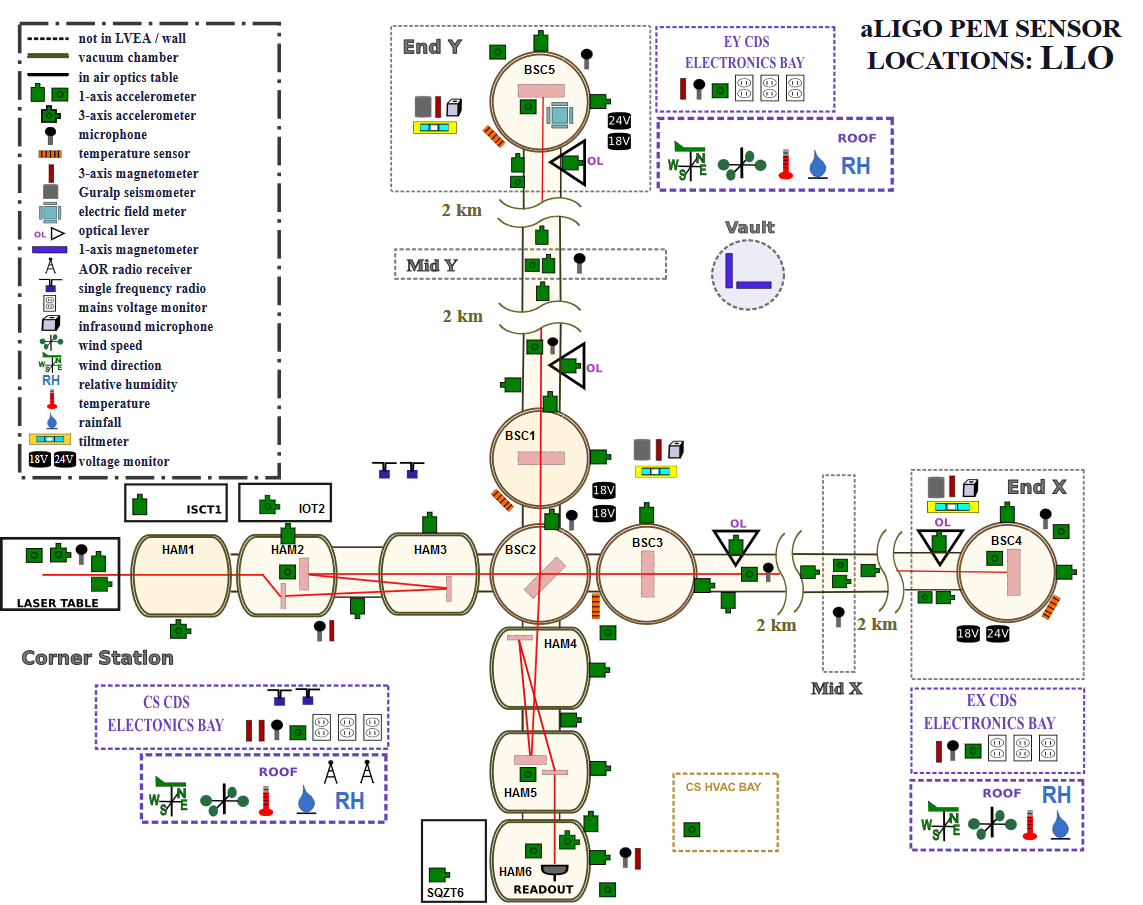
\includegraphics[width=\textwidth]{assets/llopem.png}
\caption{Schematic PEM map at the LIGO Livingston Observatory (L1). Shaded areas are in vacuum.}
\end{figure}
\begin{figure}
  \begin{minipage}[c]{0.67\textwidth}
  \begin{tabular}{c}
  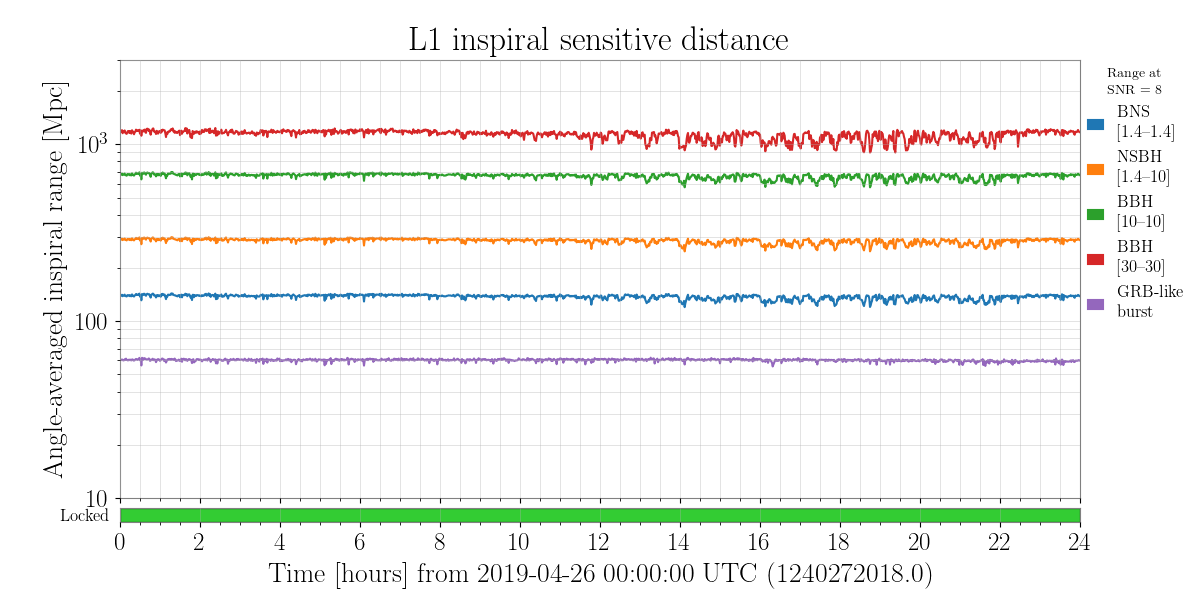
\includegraphics[width=\textwidth]{assets/L1-LOCKED_216737_RANGE-1240272018-86400.png}   \\  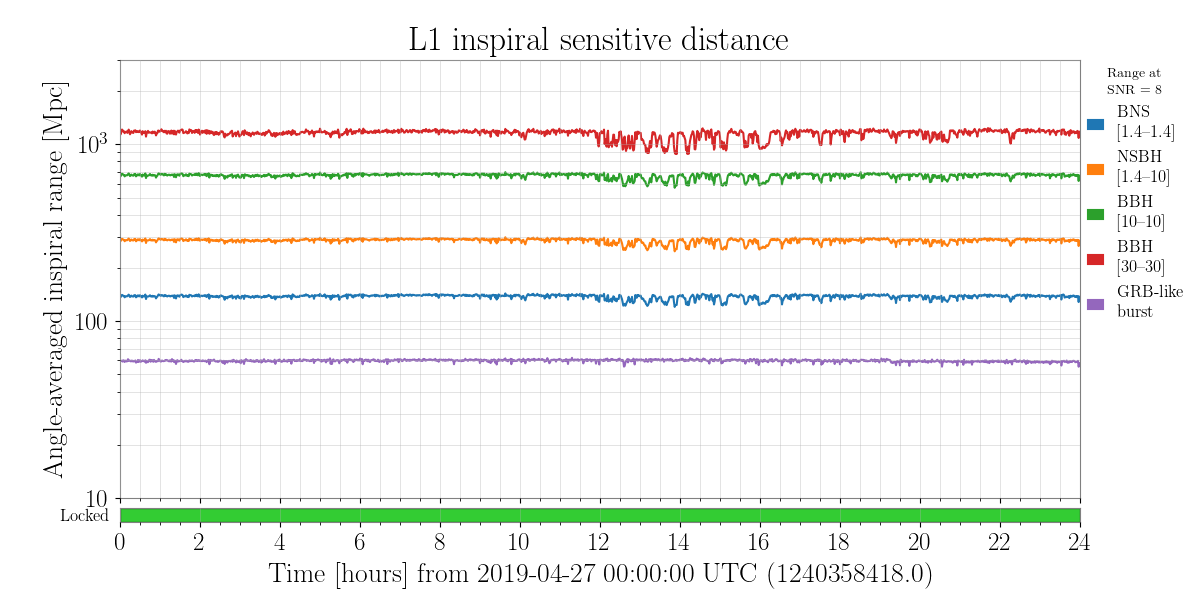
\includegraphics[width=\textwidth]{assets/L1-LOCKED_216737_RANGE-1240358418-86400.png}
  \end{tabular}
  \end{minipage}\hfill
  \begin{minipage}[t]{0.3\textwidth}
    \caption{Detector range at L1 seems to consistently reduce during the day ($\sim$6am-5pm CST). For large BBH in these plots, the reduction is about 300 Mpc. The source of this has been pinpointed to the Y end station, but the mechanism isn't fully clear.}
  \end{minipage}
\end{figure}

Separating noise sources out of a signal can be considered a clustering problem in a space covering different frequency bands in which noise appears.
A previous LIGO SURF student has evaluated several data clustering algorithms with respect to their ability to properly sort out frequency elements of seismometer signals caused by specific earthquake events\cite{roxana}.
Both the $k$-means algorithm, which aims to make clusters with low standard deviation, and the DBSCAN algorithm, which minimizes overall inter-point distance in clusters, were evaluated using multiple methods, including the Calinsky-Harabaz  index and direct comparison to earthquake times via time labeling of points, ultimately showing poor earthquake identification.
A long short-term memory (LSTM) recurrent neural network (RNN) seemed to work much better, but due to small input sample size, this solution may have been be plagued by over-fitting.
Thus, it is imperative that a more robust frequency clustering mechanism be designed for the PEM system.

\section{Objectives}
% What do you aim to accomplish in your project? What will you measure, and under what conditions; or, what will you calculate, model, or simulate; or what will you design, and what are the requirements; or what will you build or test? What is your starting point? What are your initial assumptions or conditions? What will be the result or product of a successful outcome for your project? What are the criteria for project completion or for success? (In other words, how will you know when you have accomplished what you set out to do?)
\begin{itemize}
\item
As a primary goal, \textbf{algorithms or clustering approaches which correctly identify known noise events need to be found}.
As every algorithm has inbuilt assumptions about the dataset it is applied to, the results of an algorithm performance test on labeled data will yield information about the structure of the data.
The general temporal non-stationarity of the DARM noise will need to be accounted for by varying testing time windows.
\item
The secondary goal is to \textbf{create a clustering approach to discover previously unknown noise correlations and possibly sources}.
This is where the ``detector characterization tool'' that this project aims to advance will be functional---revealing new noise coupling pathways will help identify ways to improve the detector sensitivity.
\end{itemize}

\section{Approach}
% Specifically, how will you reach your objective or produce your desired final product? What are the principal steps or milestones along the path? How long will each take? What steps promise to be the most difficult, and how will you overcome the difficulties? What equipment or other resources will you need? Which of these are inherited, and which will you have to make or procure? With what other people or groups will you be collaborating? Will completion of your project depend on results from other people in related projects? (That question may be especially pertinent for team projects.)

Initially, a program will be written to take the spectral power of any PEM channel, in the form of band-limited RMS (BLRMS), likely using established methods like looping through a smoothed spectogram of the channel\cite{vajente}.

To reach the first objective, a modular \texttt{python} testing suite will be written to probe the structure of the multidimensional frequency-domain sensor data.
This will strategically implement \texttt{scikit-learn} clustering algorithms and classifiers with different optimal regimes of function or working assumptions and evaluate them using point labeling. 
This will require, additionally to researching clustering or unsupervised classification algorithms, thinking of as many variables which may affect the data structure (such as looking at different time windows) and intelligently testing them. 
Optimizations will need to be considered so that run times are reasonable.

The program tackling the second objective will use working clustering approaches identified in the first objective to find new noise correlations.
In the event that no individual algorithm or technique outperforms the rest for all types of sensory data, the final program will use the modular programming environment created for the testing suite to match techniques to the regimes that they work in.
The structure of the input data as determined by the first objective, including the dimensionality probed by the extra variables, may lend itself to additional algorithms that can be used to combine the target regimes.
To this end, extra algorithm research will be conducted with specific consideration of the solved structure.

%%% Local Variables:
%%% mode: latex
%%% TeX-master: "../proposal"
%%% End:


\section{Interim Report 1}

In the first three weeks of the project, clustering scripts and BLRMS-generating scripts were developed and tested. Testing the clustering code on a dataset with known sources of noise was thought to be a good first-order check of its efficacy.

\subsection{$k$-means clustering with histories}
The $k$-means algorithm was used to cluster the two hours of minute-trend seismic BLRMS preceeding each point in time. Thus, each coordinate in the clustering sub-space for a channel was as follows:
\begin{equation}
  \left\{s(t_0),s(t_{-1}),s(t_{-2})\cdots,s(t_{-n})\right\}
\end{equation}

with $s(t)$ the seismometer velocity at time $t$. Each dimension corresponded to ``channel value a specific number of minutes ago''. This allowed trends over time to be matched together in a phase-agnostic way.

\begin{figure}[h]
  \tikzstyle{block} = [rectangle, draw, text width=6em, text centered, rounded corners, minimum height=4em]
  \begin{tikzpicture}[node distance = 9em, auto]
    \node [block] (dl) {get minute-trend data from NDS};
    \node [block, right of=dl] (input) {create input matrix};
    \node [block, right of=input] (compute) {compute $k$-means clusters};
    \node [block, right of=compute] (save) {save labels};
    \draw [->] (dl) -- (input);
    \draw [->] (input) -- (compute);
    \draw [->] (compute) -- (save);
  \end{tikzpicture}
  \caption{Clustering script flowchart.}
\end{figure}

For a total clustering duration of 30 days, using the seismometers attatched to ETMY, ETMX, and ITMY, in minute-trend half-order-of-magnitude BLRMS bands from 30 mHz to 30 Hz, the following known noise events were easily identified (see Figures~\ref{fig:eq}-\ref{fig:anth}):
\begin{itemize}
\item earthquakes ($0.01\to0.1$ Hz)
\item microseisms ($0.1\to1$ Hz)
\item anthropogenic noise ($1\to10$ Hz)
\end{itemize}

Some differentiation between subcategories of events in the same frequency band (e.g. earthquakes vs. wind; train vs. noise from cars) was lacking.
In the future, using unlabeled PEM data, the success of this algorithm will rely heavily on appropriate band selection.
Thinner and more targeted bands, rather than just half-order-of-magnitude, are in the works for the microphones and accelerometers.

\subsection{BLRMS-generating script}
A script to generate minute-trend BLRMS from raw PEM channels was created. This will enable BLRMS clustering for those channels not already in BLRMS frames.

\begin{figure}[h]
  \tikzstyle{block} = [rectangle, draw, text width=6em, text centered, rounded corners, minimum height=4em]
  \begin{tikzpicture}[node distance = 9em, auto]
    \node [block] (dl) {get raw data from NDS};
    \node [block, below of=dl] (strides) {compute strides};
    \node [block, right of=strides] (next) {get next stride};
    \node [block, below of=next] (stride) {extract stride};
    \node [block, right of=stride] (compute) {compute spectogram};
    \node [block, right of=compute] (add) {add power within requested bands};
    \node [block, right of=add] (save) {stitch stride into .hdf5 file};
    \node [block, below of=add] (shape) {read .hdf5 dataset shape};
    \node [block, below of=save] (offset) {compute offset};
    \draw [->] (dl) -- (strides);
    \draw [->] (strides) -- (next);
    \draw [->] (next) -- (stride);
    \draw [->] (stride) -- (compute);
    \draw [->] (compute) -- (add);
    \draw [->] (add) -- (save);
    \draw [->] (stride) |- (shape);
    \draw [->] (shape) -- (offset);
    \draw [->] (offset) -- (save);
    \draw [->] (save) |- (next);
  \end{tikzpicture}
  \caption{BLRMS script flowchart.}
\end{figure}

\begin{figure}
  \begin{minipage}[t]{0.3\textwidth}
    \caption{Examples of earthquakes. These vary most of all seismic noise events, so most of the extra, unrequired clusters tend to pick details out in these. For instance, two different kinds of earthquakes were picked up (here orange and purple predominantly).}\label{fig:eq}
  \end{minipage}\hfill
  \begin{minipage}[c]{0.67\textwidth}
    \begin{tabular}{c}
      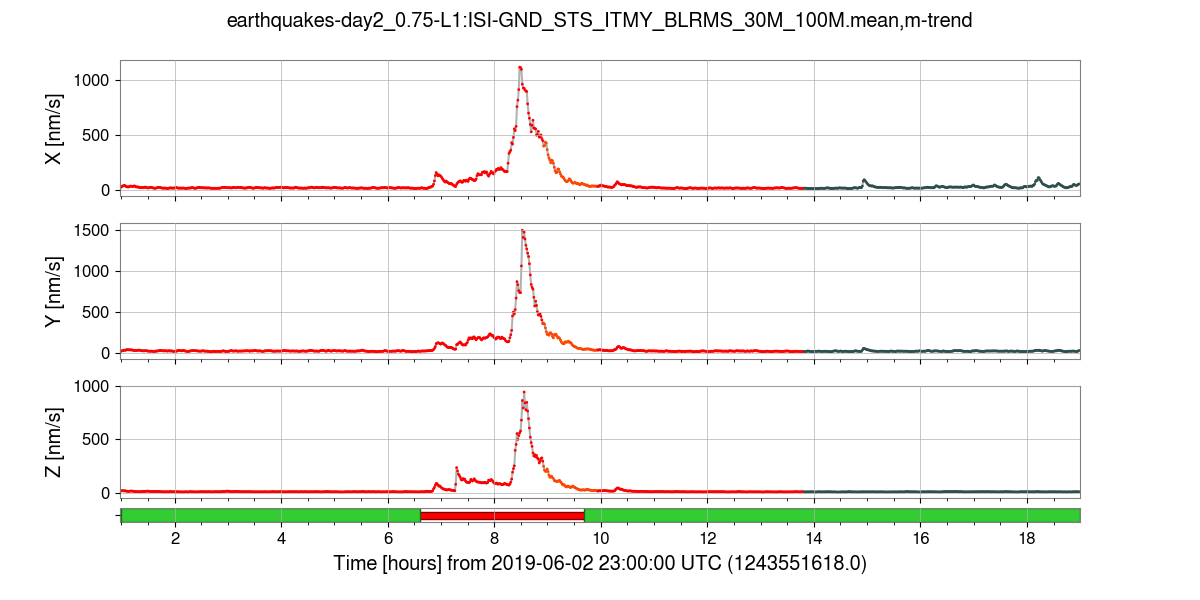
\includegraphics[width=\textwidth]{assets/report1/earthquakes-day2_075-L1:ISI-GND_STS_ITMY_BLRMS_30M_100Mmean,m-trend.png}\\
      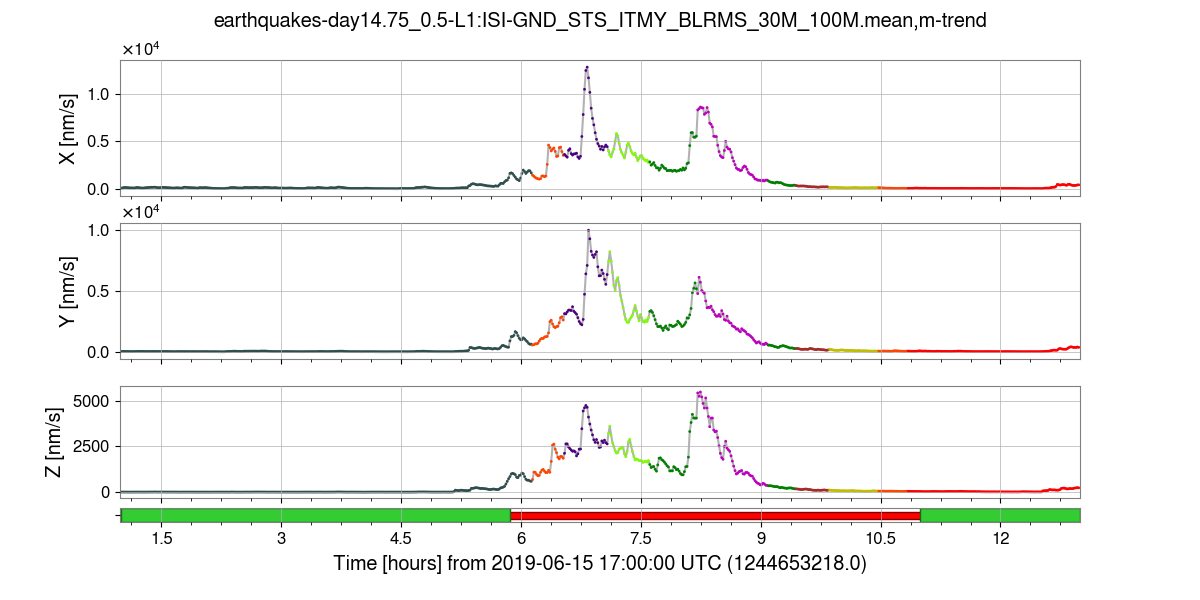
\includegraphics[width=\textwidth]{assets/report1/earthquakes-day1475_05-L1:ISI-GND_STS_ITMY_BLRMS_30M_100Mmean,m-trend.png}\\
      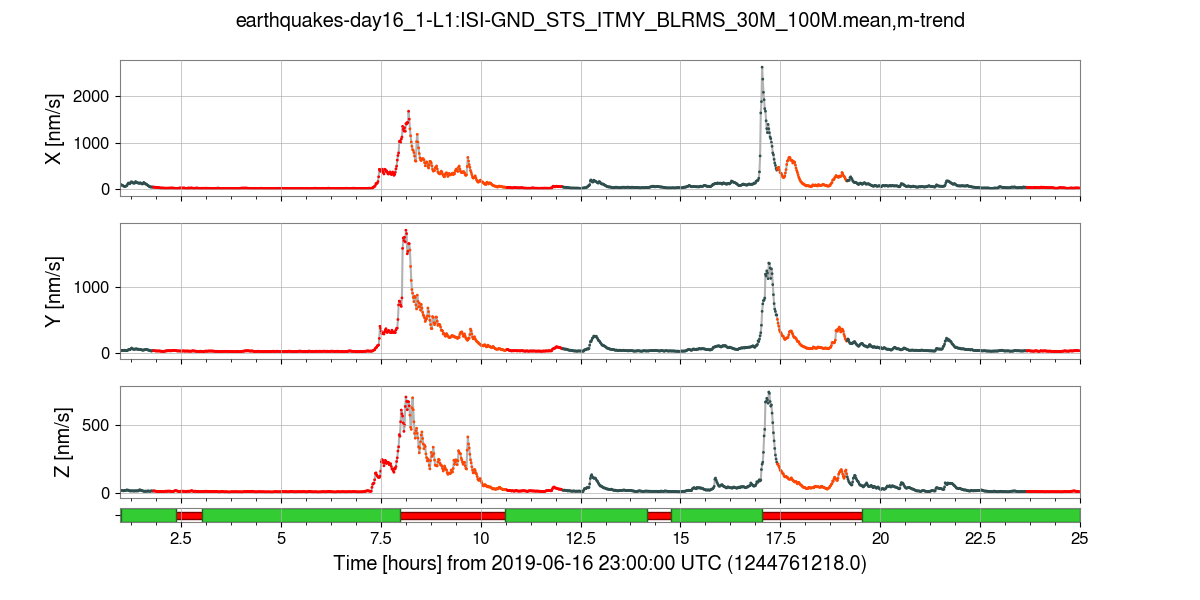
\includegraphics[width=\textwidth]{assets/report1/earthquakes-day16_1-L1:ISI-GND_STS_ITMY_BLRMS_30M_100Mmean,m-trend.png}\\
      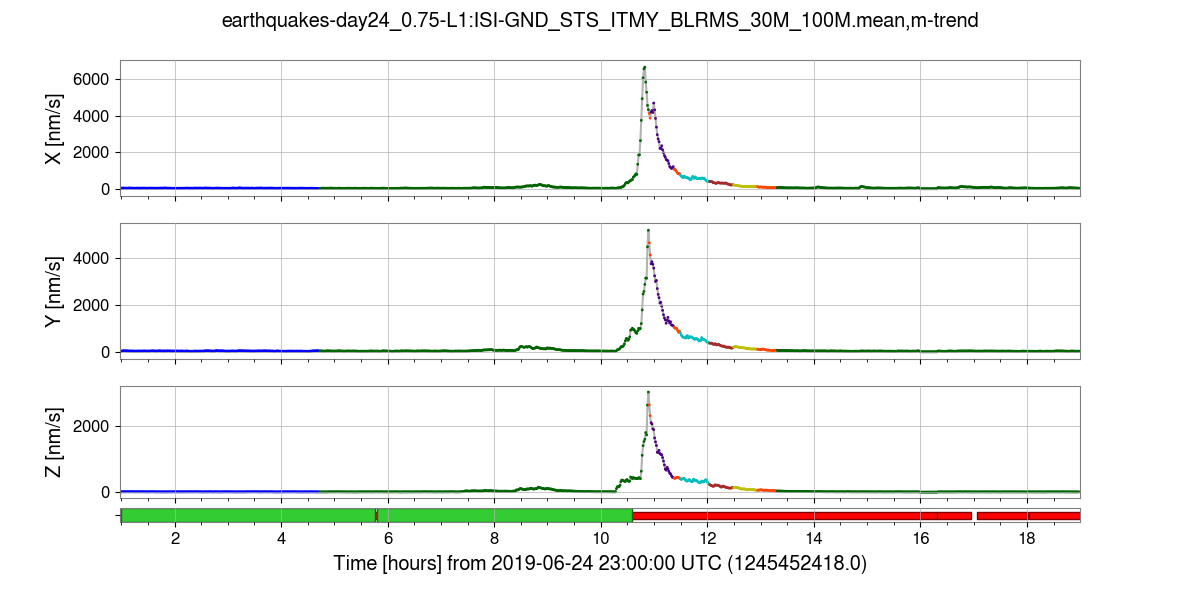
\includegraphics[width=\textwidth]{assets/report1/earthquakes-day24_075-L1:ISI-GND_STS_ITMY_BLRMS_30M_100Mmean,m-trend.png}
    \end{tabular}
  \end{minipage}
\end{figure}

\begin{figure}
  \begin{minipage}[c]{0.67\textwidth}
    \begin{tabular}{c}
      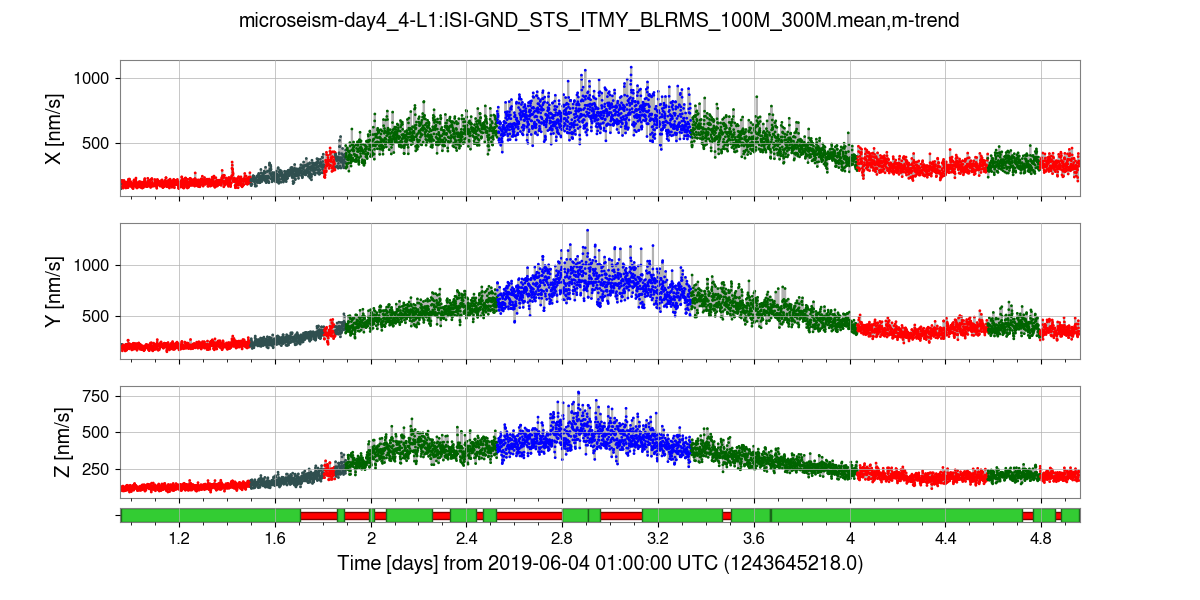
\includegraphics[width=\textwidth]{assets/report1/microseism-day4_4-L1:ISI-GND_STS_ITMY_BLRMS_100M_300Mmean,m-trend.png}\\
      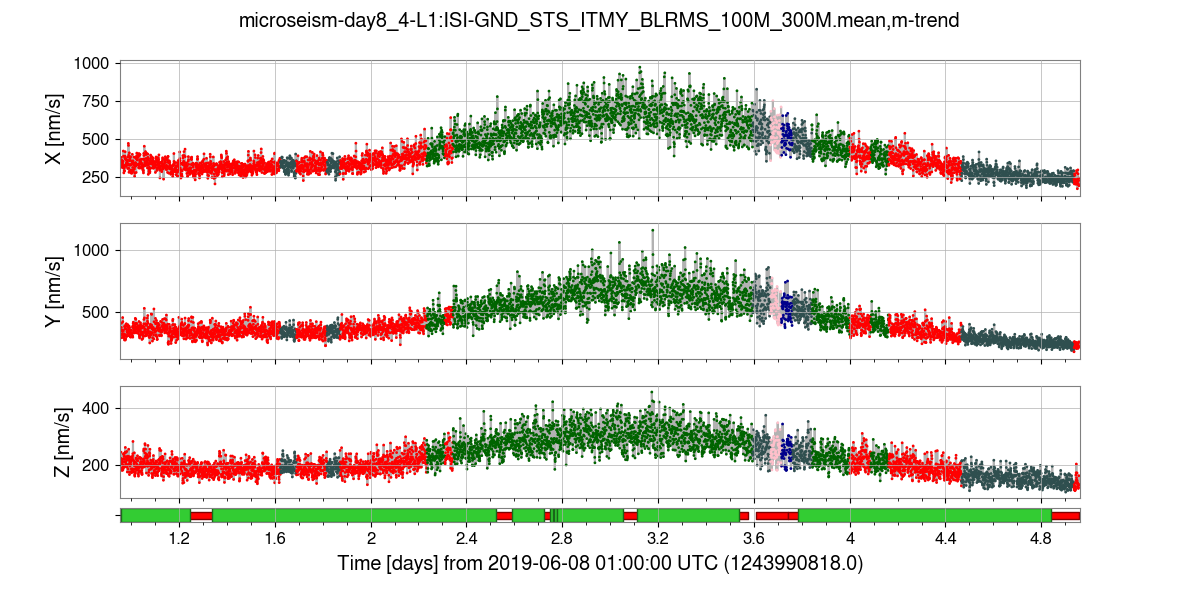
\includegraphics[width=\textwidth]{assets/report1/microseism-day8_4-L1:ISI-GND_STS_ITMY_BLRMS_100M_300Mmean,m-trend.png}\\
      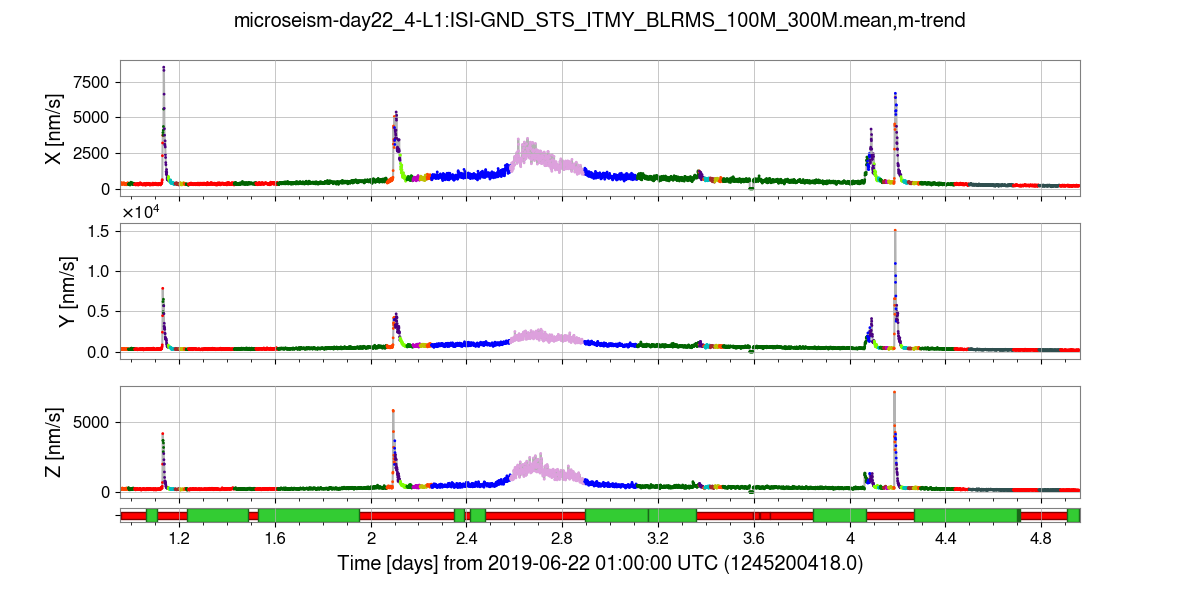
\includegraphics[width=\textwidth]{assets/report1/microseism-day22_4-L1:ISI-GND_STS_ITMY_BLRMS_100M_300Mmean,m-trend.png}
    \end{tabular}
  \end{minipage}\hfill
  \begin{minipage}[t]{0.3\textwidth}
    \caption{Examples of microseisms identified by the k-means algorithm. Because the algorithm was run with more clusters than needed, several clusters are assigned to this class of event. Running with less clusters fixes this issue, but details are sometimes missed.}
  \end{minipage}
\end{figure}


\begin{figure}
  \begin{minipage}[t]{0.3\textwidth}
    \caption{Day-night anthropogenic noise variation is identified by the k-means algorithm. These clusters are depicted grey.}
  \end{minipage}\hfill
  \begin{minipage}[c]{0.67\textwidth}
    \begin{tabular}{c}
      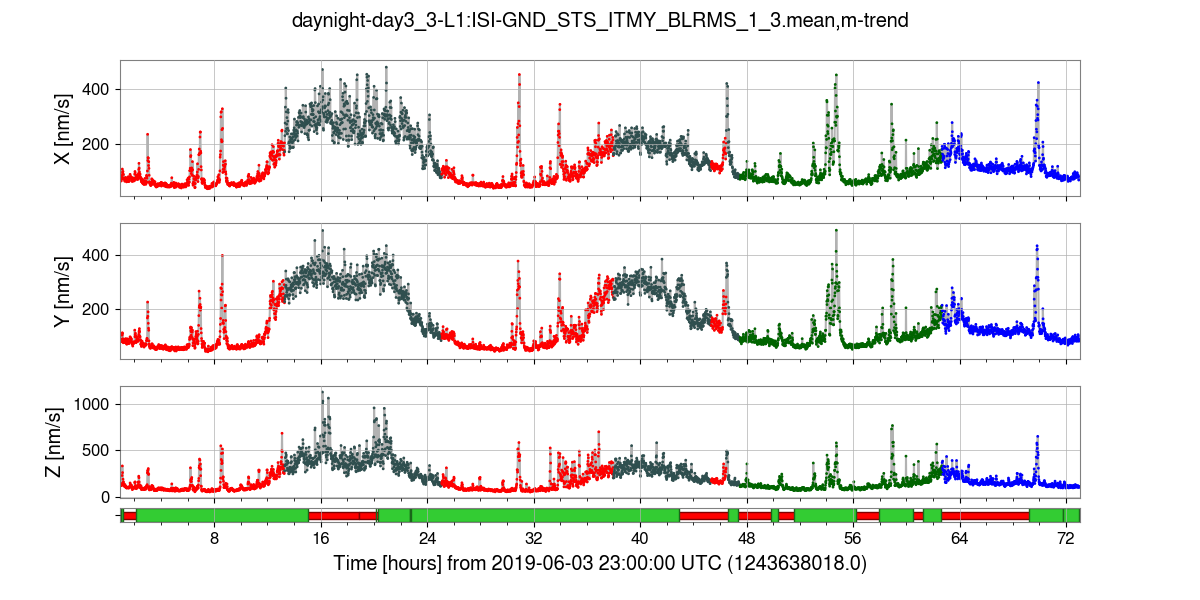
\includegraphics[width=\textwidth]{assets/report1/daynight-day3_3-L1:ISI-GND_STS_ITMY_BLRMS_1_3mean,m-trend.png}\\
      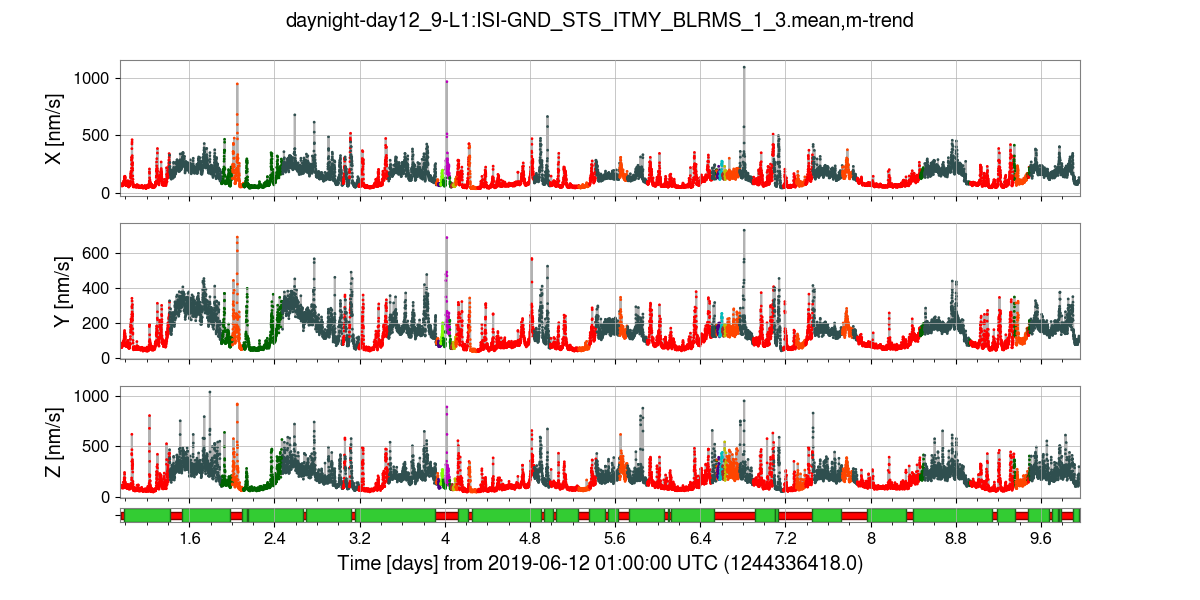
\includegraphics[width=\textwidth]{assets/report1/daynight-day12_9-L1:ISI-GND_STS_ITMY_BLRMS_1_3mean,m-trend.png}
    \end{tabular}
  \end{minipage}
\end{figure}

\begin{figure}
  \begin{minipage}[c]{0.67\textwidth}
    \begin{tabular}{c}
      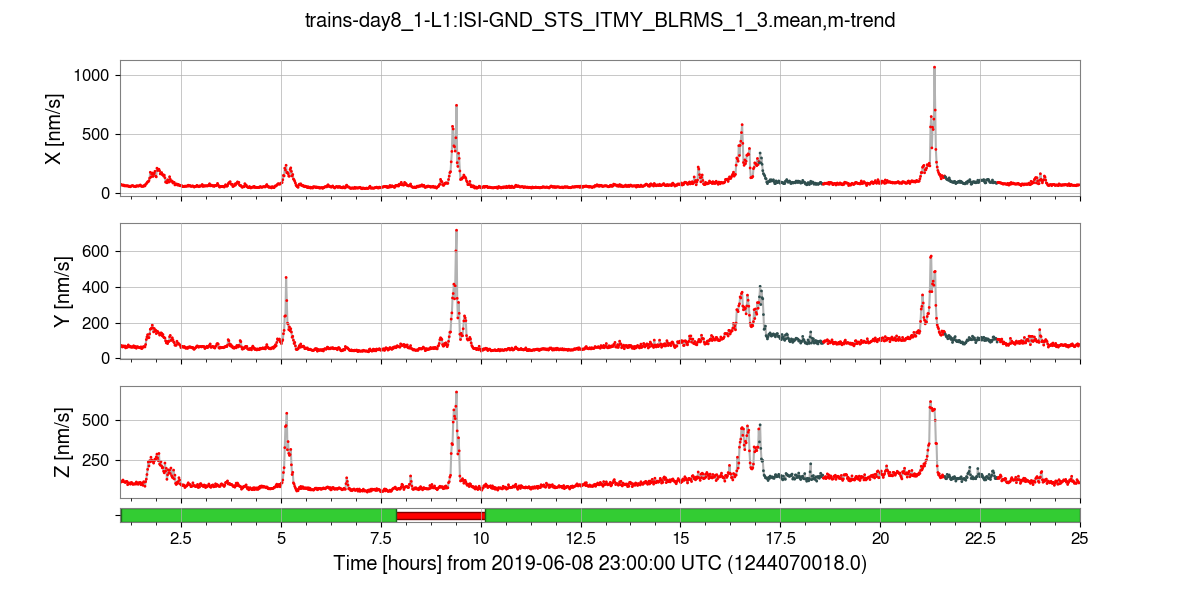
\includegraphics[width=\textwidth]{assets/report1/trains-day8_1-L1:ISI-GND_STS_ITMY_BLRMS_1_3mean,m-trend.png}\\
      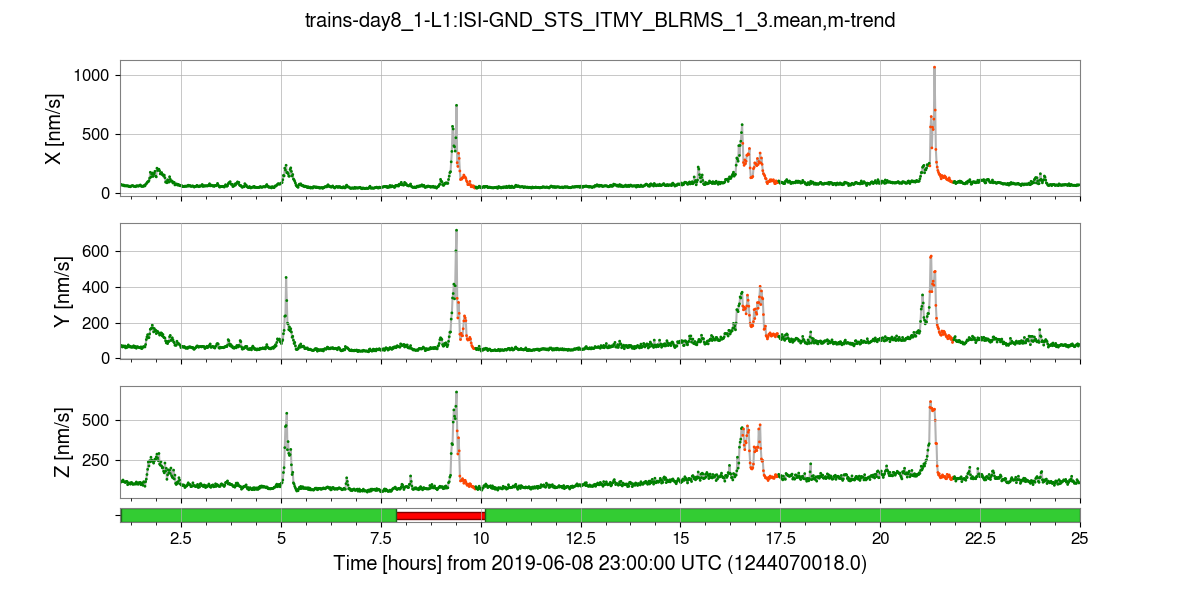
\includegraphics[width=\textwidth]{assets/report1/30m-trains-day8_1-L1:ISI-GND_STS_ITMY_BLRMS_1_3mean,m-trend.png}
    \end{tabular}
  \end{minipage}\hfill
  \begin{minipage}[t]{0.3\textwidth}
    \caption{Trains are clustered with the day/night anthropogenic noise. Shortening the history window from 2 hours (upper) to 30 minutes (lower)  helps to clarify this.}\label{fig:anth}
  \end{minipage}
\end{figure}

\begin{thebibliography}{2}
\bibitem{aepaper} A. Effler, R. M. S. Schofield, V. V. Frolov, G. Gonz{\'{a}}lez, K. Kawabe, J. R. Smith, J. Birch, and R. McCarthy, Classical and Quantum Gravity \textbf{32}, 035017 (2015).
\bibitem{roxana} LIGO Document T1700198-v1
\bibitem{vajente} aLIGO LLO Logbook entry 45374 by Gabriele Vajente
\end{thebibliography}



\end{document}

